\chapter{Экспериментальный раздел}
\label{cha:research}
    В данном разделе будут проведены эксперименты для проведения 
    сравнительного анализа алгоритмов по затрачиваемому процессорному 
    времени\cite{CPU-time}.
% и количеству максимально затрачиваемой памяти
    \section{Сравнительный анализ на основе замеров времени работы алгоритмов}
    
        Был проведён замер времени работы каждого из алгоритмов:
        
        1) на небольших длинах строк (рисунок \ref{png:test:1});
        
        2) на относительно больших длинах строк (рисунок \ref{png:test:2}).
        
        Ниже предствалены графики полученных замеров времени
        (диаграммы \ref{diag:test:1} и \ref{diag:test:2}).

        \begin{figure}[h!]
            \centering
            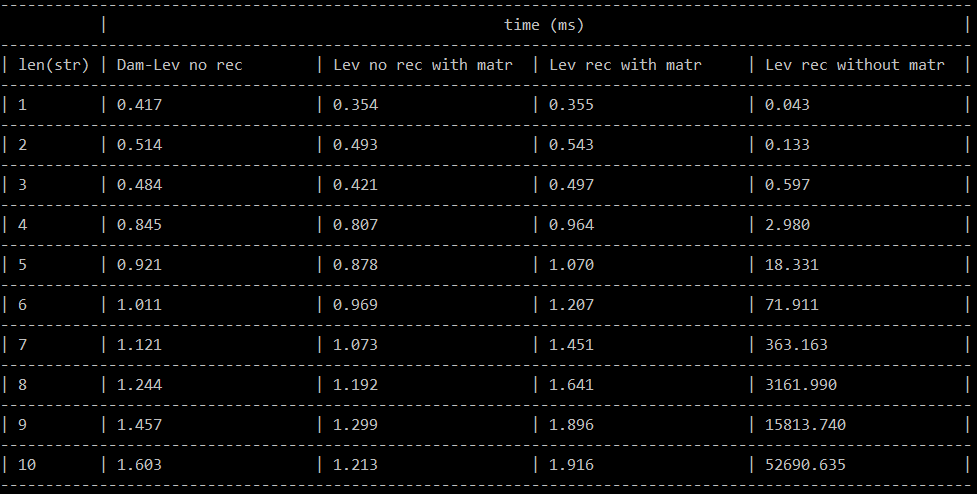
\includegraphics[scale=0.7]{test1.png}
            \caption{Результаты замера времени на маленьких строках}
            \label{png:test:1}

            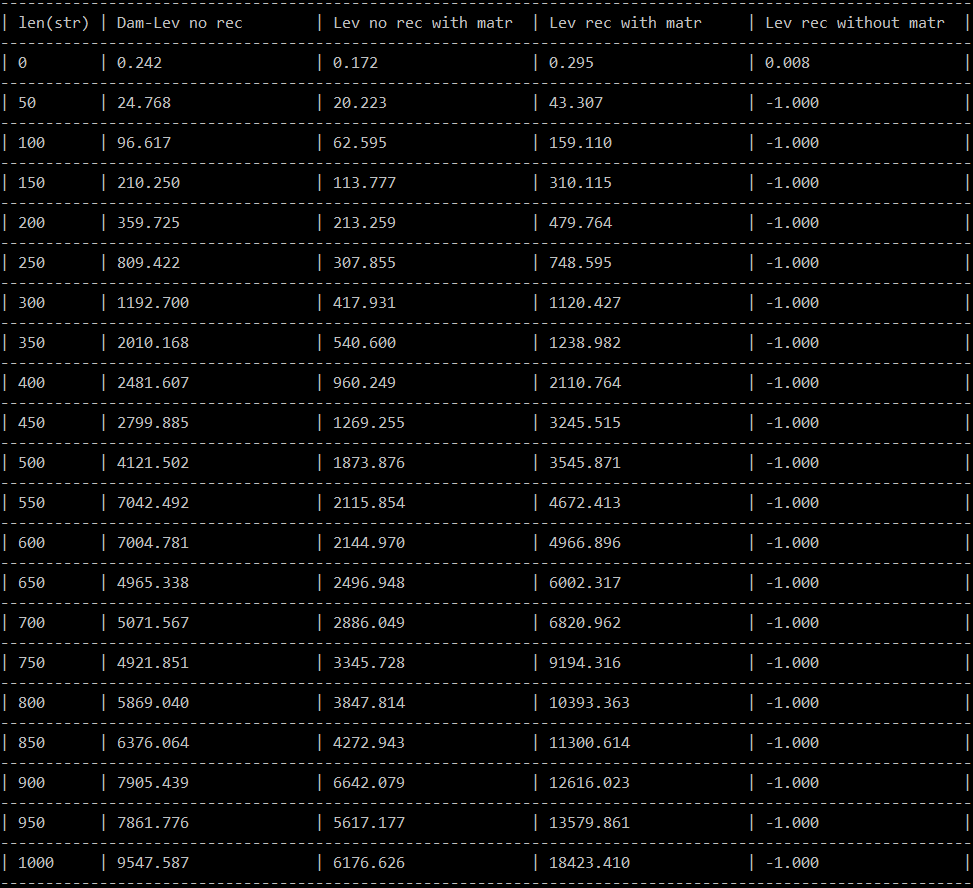
\includegraphics[scale=0.7]{test2.png}
            \caption{Результаты замера времени на больших строках}
            \label{png:test:2}
        \end{figure}

        \begin{figure}[h!]
            \centering
            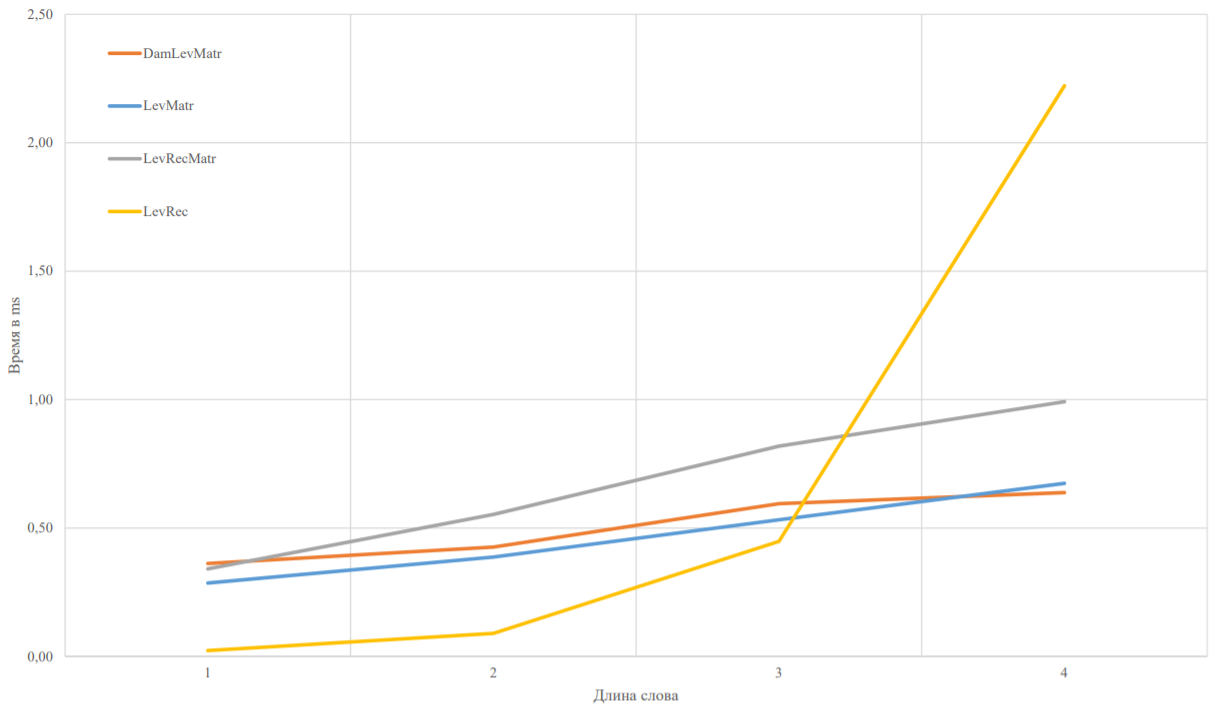
\includegraphics[scale=0.7]{diagram1.png}
            \caption{Зависимость времени работы алгоритма от длины малых строк}
            \label{diag:test:1}
            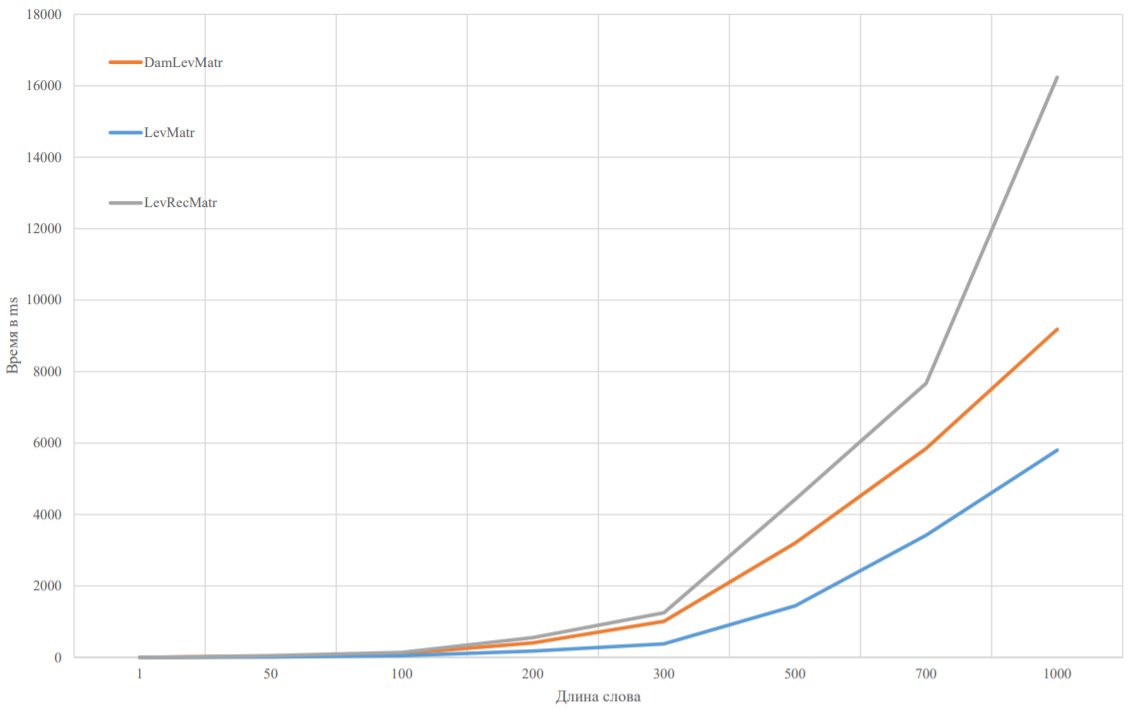
\includegraphics[scale=0.7]{diagram2.png}
            \caption{Зависимость времени работы алгоритма от длины больших строк}
            \label{diag:test:2}
        \end{figure}
\newpage